\documentclass[tikz]{standalone}

\usetikzlibrary{decorations.pathmorphing,patterns,calc}

\begin{document}
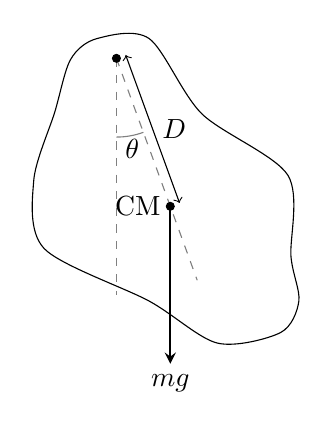
\begin{tikzpicture}
		\def\centerarc[#1](#2)(#3:#4:#5)% Syntax: [draw options] (center) (initial angle:final angle:radius)
		{ \draw[#1] ($(#2)+({#5*cos(#3)},{#5*sin(#3)})$) arc (#3:#4:#5); }
		
		\coordinate (origin) at (0.25, -0.25);
		\path (origin) + (-70:2) coordinate (cm);
		
		% Body
		\draw [fill=white] plot [smooth cycle, solid] coordinates { (0,0) (1/1.5,0) (2/1.5, -1.43/1.5) (3.64/1.5, -2.6/1.5) (3.7/1.5, -4.15/1.5) (3.85/1.5,-5/1.5) (3.5/1.5, -5.6/1.5) (2.3/1.5, -5.8/1.5) (1/1.5, -5/1.5) (-1/1.5, -4/1.5) (-1.2/1.5, -2.7/1.5) (-0.8/1.5,-1.4/1.5) (-0.5/1.5, -0.4/1.5) };
		
		%Dashed lines
		\draw [gray, dashed] (origin) -- ++(-70:3);
		\draw [gray, dashed] (origin) -- ++(-90:3);
		
		% Circles
		\draw [fill=black] (origin) circle (0.05);
		\draw [fill=black] (cm) circle (0.05) node[left] {CM};
		
		% Force
		\draw[-stealth,thick] (cm) -- ++(-90:2) node[below] {$mg$};
		
		%Angle
		\centerarc[gray](origin)(-90:-70:1)
		\node at (0.45,-1.4) {$\theta$};
		
		% Distance
		\path (origin) + (20:0.125) coordinate (start);
		\path (cm) + (20:0.125) coordinate (end);
		\draw[<->] (start) -- (end);
		\path (start) + (-70:1) coordinate (distance);
		\node [right] at (distance) {$D$};
	\end{tikzpicture}
\end{document}